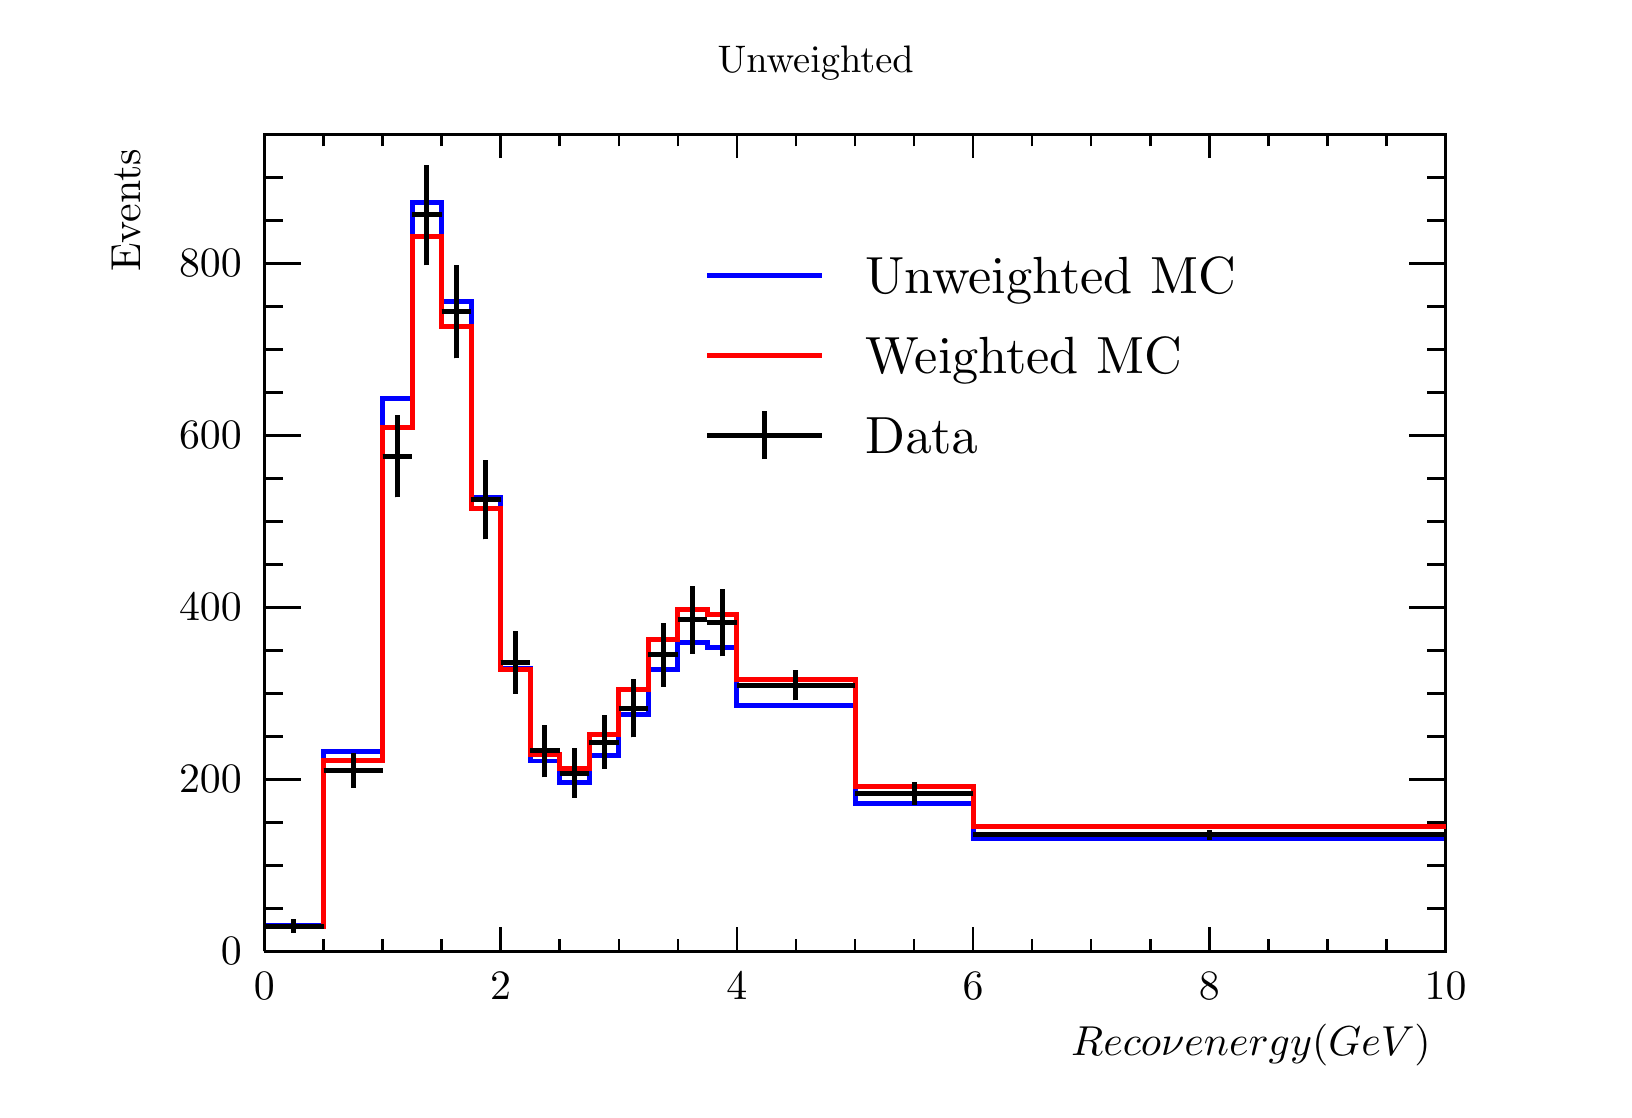
\begin{tikzpicture}
\pgfdeclareplotmark{cross} {
\pgfpathmoveto{\pgfpoint{-0.3\pgfplotmarksize}{\pgfplotmarksize}}
\pgfpathlineto{\pgfpoint{+0.3\pgfplotmarksize}{\pgfplotmarksize}}
\pgfpathlineto{\pgfpoint{+0.3\pgfplotmarksize}{0.3\pgfplotmarksize}}
\pgfpathlineto{\pgfpoint{+1\pgfplotmarksize}{0.3\pgfplotmarksize}}
\pgfpathlineto{\pgfpoint{+1\pgfplotmarksize}{-0.3\pgfplotmarksize}}
\pgfpathlineto{\pgfpoint{+0.3\pgfplotmarksize}{-0.3\pgfplotmarksize}}
\pgfpathlineto{\pgfpoint{+0.3\pgfplotmarksize}{-1.\pgfplotmarksize}}
\pgfpathlineto{\pgfpoint{-0.3\pgfplotmarksize}{-1.\pgfplotmarksize}}
\pgfpathlineto{\pgfpoint{-0.3\pgfplotmarksize}{-0.3\pgfplotmarksize}}
\pgfpathlineto{\pgfpoint{-1.\pgfplotmarksize}{-0.3\pgfplotmarksize}}
\pgfpathlineto{\pgfpoint{-1.\pgfplotmarksize}{0.3\pgfplotmarksize}}
\pgfpathlineto{\pgfpoint{-0.3\pgfplotmarksize}{0.3\pgfplotmarksize}}
\pgfpathclose
\pgfusepathqstroke
}
\pgfdeclareplotmark{cross*} {
\pgfpathmoveto{\pgfpoint{-0.3\pgfplotmarksize}{\pgfplotmarksize}}
\pgfpathlineto{\pgfpoint{+0.3\pgfplotmarksize}{\pgfplotmarksize}}
\pgfpathlineto{\pgfpoint{+0.3\pgfplotmarksize}{0.3\pgfplotmarksize}}
\pgfpathlineto{\pgfpoint{+1\pgfplotmarksize}{0.3\pgfplotmarksize}}
\pgfpathlineto{\pgfpoint{+1\pgfplotmarksize}{-0.3\pgfplotmarksize}}
\pgfpathlineto{\pgfpoint{+0.3\pgfplotmarksize}{-0.3\pgfplotmarksize}}
\pgfpathlineto{\pgfpoint{+0.3\pgfplotmarksize}{-1.\pgfplotmarksize}}
\pgfpathlineto{\pgfpoint{-0.3\pgfplotmarksize}{-1.\pgfplotmarksize}}
\pgfpathlineto{\pgfpoint{-0.3\pgfplotmarksize}{-0.3\pgfplotmarksize}}
\pgfpathlineto{\pgfpoint{-1.\pgfplotmarksize}{-0.3\pgfplotmarksize}}
\pgfpathlineto{\pgfpoint{-1.\pgfplotmarksize}{0.3\pgfplotmarksize}}
\pgfpathlineto{\pgfpoint{-0.3\pgfplotmarksize}{0.3\pgfplotmarksize}}
\pgfpathclose
\pgfusepathqfillstroke
}
\pgfdeclareplotmark{newstar} {
\pgfpathmoveto{\pgfqpoint{0pt}{\pgfplotmarksize}}
\pgfpathlineto{\pgfqpointpolar{44}{0.5\pgfplotmarksize}}
\pgfpathlineto{\pgfqpointpolar{18}{\pgfplotmarksize}}
\pgfpathlineto{\pgfqpointpolar{-20}{0.5\pgfplotmarksize}}
\pgfpathlineto{\pgfqpointpolar{-54}{\pgfplotmarksize}}
\pgfpathlineto{\pgfqpointpolar{-90}{0.5\pgfplotmarksize}}
\pgfpathlineto{\pgfqpointpolar{234}{\pgfplotmarksize}}
\pgfpathlineto{\pgfqpointpolar{198}{0.5\pgfplotmarksize}}
\pgfpathlineto{\pgfqpointpolar{162}{\pgfplotmarksize}}
\pgfpathlineto{\pgfqpointpolar{134}{0.5\pgfplotmarksize}}
\pgfpathclose
\pgfusepathqstroke
}
\pgfdeclareplotmark{newstar*} {
\pgfpathmoveto{\pgfqpoint{0pt}{\pgfplotmarksize}}
\pgfpathlineto{\pgfqpointpolar{44}{0.5\pgfplotmarksize}}
\pgfpathlineto{\pgfqpointpolar{18}{\pgfplotmarksize}}
\pgfpathlineto{\pgfqpointpolar{-20}{0.5\pgfplotmarksize}}
\pgfpathlineto{\pgfqpointpolar{-54}{\pgfplotmarksize}}
\pgfpathlineto{\pgfqpointpolar{-90}{0.5\pgfplotmarksize}}
\pgfpathlineto{\pgfqpointpolar{234}{\pgfplotmarksize}}
\pgfpathlineto{\pgfqpointpolar{198}{0.5\pgfplotmarksize}}
\pgfpathlineto{\pgfqpointpolar{162}{\pgfplotmarksize}}
\pgfpathlineto{\pgfqpointpolar{134}{0.5\pgfplotmarksize}}
\pgfpathclose
\pgfusepathqfillstroke
}
\definecolor{c}{rgb}{1,1,1};
\draw [color=c, fill=c] (0,0) rectangle (20,13.4752);
\draw [color=c, fill=c] (3,1.75177) rectangle (18,12.1277);
\definecolor{c}{rgb}{0,0,0};
\draw [c,line width=0.9] (3,1.75177) -- (3,12.1277) -- (18,12.1277) -- (18,1.75177) -- (3,1.75177);
\definecolor{c}{rgb}{1,1,1};
\draw [color=c, fill=c] (3,1.75177) rectangle (18,12.1277);
\definecolor{c}{rgb}{0,0,0};
\draw [c,line width=0.9] (3,1.75177) -- (3,12.1277) -- (18,12.1277) -- (18,1.75177) -- (3,1.75177);
\definecolor{c}{rgb}{0,0,1};
\draw [c,line width=1.8] (3,2.07958) -- (3.75,2.07958) -- (3.75,4.28523) -- (4.5,4.28523) -- (4.5,8.77265) -- (4.875,8.77265) -- (4.875,11.2649) -- (5.25,11.2649) -- (5.25,10.0098) -- (5.625,10.0098) -- (5.625,7.51667) -- (6,7.51667) -- (6,5.34596)
 -- (6.375,5.34596) -- (6.375,4.16897) -- (6.75,4.16897) -- (6.75,3.8993) -- (7.125,3.8993) -- (7.125,4.24495) -- (7.5,4.24495) -- (7.5,4.76016) -- (7.875,4.76016) -- (7.875,5.33064) -- (8.25,5.33064) -- (8.25,5.67974) -- (8.625,5.67974) --
 (8.625,5.6107) -- (9,5.6107) -- (9,4.86975) -- (10.5,4.86975) -- (10.5,3.62597) -- (12,3.62597) -- (12,3.18824) -- (18,3.18824);
\definecolor{c}{rgb}{0,0,0};
\draw [c,line width=0.9] (3,1.75177) -- (18,1.75177);
\draw [c,line width=0.9] (3,2.05496) -- (3,1.75177);
\draw [c,line width=0.9] (3.75,1.90337) -- (3.75,1.75177);
\draw [c,line width=0.9] (4.5,1.90337) -- (4.5,1.75177);
\draw [c,line width=0.9] (5.25,1.90337) -- (5.25,1.75177);
\draw [c,line width=0.9] (6,2.05496) -- (6,1.75177);
\draw [c,line width=0.9] (6.75,1.90337) -- (6.75,1.75177);
\draw [c,line width=0.9] (7.5,1.90337) -- (7.5,1.75177);
\draw [c,line width=0.9] (8.25,1.90337) -- (8.25,1.75177);
\draw [c,line width=0.9] (9,2.05496) -- (9,1.75177);
\draw [c,line width=0.9] (9.75,1.90337) -- (9.75,1.75177);
\draw [c,line width=0.9] (10.5,1.90337) -- (10.5,1.75177);
\draw [c,line width=0.9] (11.25,1.90337) -- (11.25,1.75177);
\draw [c,line width=0.9] (12,2.05496) -- (12,1.75177);
\draw [c,line width=0.9] (12.75,1.90337) -- (12.75,1.75177);
\draw [c,line width=0.9] (13.5,1.90337) -- (13.5,1.75177);
\draw [c,line width=0.9] (14.25,1.90337) -- (14.25,1.75177);
\draw [c,line width=0.9] (15,2.05496) -- (15,1.75177);
\draw [c,line width=0.9] (15.75,1.90337) -- (15.75,1.75177);
\draw [c,line width=0.9] (16.5,1.90337) -- (16.5,1.75177);
\draw [c,line width=0.9] (17.25,1.90337) -- (17.25,1.75177);
\draw [c,line width=0.9] (18,2.05496) -- (18,1.75177);
\draw [anchor=base] (3,1.14539) node[scale=1.51215, color=c, rotate=0]{0};
\draw [anchor=base] (6,1.14539) node[scale=1.51215, color=c, rotate=0]{2};
\draw [anchor=base] (9,1.14539) node[scale=1.51215, color=c, rotate=0]{4};
\draw [anchor=base] (12,1.14539) node[scale=1.51215, color=c, rotate=0]{6};
\draw [anchor=base] (15,1.14539) node[scale=1.51215, color=c, rotate=0]{8};
\draw [anchor=base] (18,1.14539) node[scale=1.51215, color=c, rotate=0]{10};
\draw [anchor= east] (18,0.565957) node[scale=1.51215, color=c, rotate=0]{$Reco \nu energy (GeV)$};
\draw [c,line width=0.9] (3,12.1277) -- (18,12.1277);
\draw [c,line width=0.9] (3,11.8245) -- (3,12.1277);
\draw [c,line width=0.9] (3.75,11.9761) -- (3.75,12.1277);
\draw [c,line width=0.9] (4.5,11.9761) -- (4.5,12.1277);
\draw [c,line width=0.9] (5.25,11.9761) -- (5.25,12.1277);
\draw [c,line width=0.9] (6,11.8245) -- (6,12.1277);
\draw [c,line width=0.9] (6.75,11.9761) -- (6.75,12.1277);
\draw [c,line width=0.9] (7.5,11.9761) -- (7.5,12.1277);
\draw [c,line width=0.9] (8.25,11.9761) -- (8.25,12.1277);
\draw [c,line width=0.9] (9,11.8245) -- (9,12.1277);
\draw [c,line width=0.9] (9.75,11.9761) -- (9.75,12.1277);
\draw [c,line width=0.9] (10.5,11.9761) -- (10.5,12.1277);
\draw [c,line width=0.9] (11.25,11.9761) -- (11.25,12.1277);
\draw [c,line width=0.9] (12,11.8245) -- (12,12.1277);
\draw [c,line width=0.9] (12.75,11.9761) -- (12.75,12.1277);
\draw [c,line width=0.9] (13.5,11.9761) -- (13.5,12.1277);
\draw [c,line width=0.9] (14.25,11.9761) -- (14.25,12.1277);
\draw [c,line width=0.9] (15,11.8245) -- (15,12.1277);
\draw [c,line width=0.9] (15.75,11.9761) -- (15.75,12.1277);
\draw [c,line width=0.9] (16.5,11.9761) -- (16.5,12.1277);
\draw [c,line width=0.9] (17.25,11.9761) -- (17.25,12.1277);
\draw [c,line width=0.9] (18,11.8245) -- (18,12.1277);
\draw [c,line width=0.9] (3,1.75177) -- (3,12.1277);
\draw [c,line width=0.9] (3.462,1.75177) -- (3,1.75177);
\draw [c,line width=0.9] (3.231,2.29787) -- (3,2.29787);
\draw [c,line width=0.9] (3.231,2.84397) -- (3,2.84397);
\draw [c,line width=0.9] (3.231,3.39007) -- (3,3.39007);
\draw [c,line width=0.9] (3.462,3.93617) -- (3,3.93617);
\draw [c,line width=0.9] (3.231,4.48227) -- (3,4.48227);
\draw [c,line width=0.9] (3.231,5.02837) -- (3,5.02837);
\draw [c,line width=0.9] (3.231,5.57447) -- (3,5.57447);
\draw [c,line width=0.9] (3.462,6.12057) -- (3,6.12057);
\draw [c,line width=0.9] (3.231,6.66667) -- (3,6.66667);
\draw [c,line width=0.9] (3.231,7.21277) -- (3,7.21277);
\draw [c,line width=0.9] (3.231,7.75887) -- (3,7.75887);
\draw [c,line width=0.9] (3.462,8.30497) -- (3,8.30497);
\draw [c,line width=0.9] (3.231,8.85106) -- (3,8.85106);
\draw [c,line width=0.9] (3.231,9.39716) -- (3,9.39716);
\draw [c,line width=0.9] (3.231,9.94326) -- (3,9.94326);
\draw [c,line width=0.9] (3.462,10.4894) -- (3,10.4894);
\draw [c,line width=0.9] (3.462,10.4894) -- (3,10.4894);
\draw [c,line width=0.9] (3.231,11.0355) -- (3,11.0355);
\draw [c,line width=0.9] (3.231,11.5816) -- (3,11.5816);
\draw [c,line width=0.9] (3.231,12.1277) -- (3,12.1277);
\draw [anchor= east] (2.9,1.75177) node[scale=1.51215, color=c, rotate=0]{0};
\draw [anchor= east] (2.9,3.93617) node[scale=1.51215, color=c, rotate=0]{200};
\draw [anchor= east] (2.9,6.12057) node[scale=1.51215, color=c, rotate=0]{400};
\draw [anchor= east] (2.9,8.30497) node[scale=1.51215, color=c, rotate=0]{600};
\draw [anchor= east] (2.9,10.4894) node[scale=1.51215, color=c, rotate=0]{800};
\draw [anchor= east] (1.24,12.1277) node[scale=1.51215, color=c, rotate=90]{Events};
\draw [c,line width=0.9] (18,1.75177) -- (18,12.1277);
\draw [c,line width=0.9] (17.538,1.75177) -- (18,1.75177);
\draw [c,line width=0.9] (17.769,2.29787) -- (18,2.29787);
\draw [c,line width=0.9] (17.769,2.84397) -- (18,2.84397);
\draw [c,line width=0.9] (17.769,3.39007) -- (18,3.39007);
\draw [c,line width=0.9] (17.538,3.93617) -- (18,3.93617);
\draw [c,line width=0.9] (17.769,4.48227) -- (18,4.48227);
\draw [c,line width=0.9] (17.769,5.02837) -- (18,5.02837);
\draw [c,line width=0.9] (17.769,5.57447) -- (18,5.57447);
\draw [c,line width=0.9] (17.538,6.12057) -- (18,6.12057);
\draw [c,line width=0.9] (17.769,6.66667) -- (18,6.66667);
\draw [c,line width=0.9] (17.769,7.21277) -- (18,7.21277);
\draw [c,line width=0.9] (17.769,7.75887) -- (18,7.75887);
\draw [c,line width=0.9] (17.538,8.30497) -- (18,8.30497);
\draw [c,line width=0.9] (17.769,8.85106) -- (18,8.85106);
\draw [c,line width=0.9] (17.769,9.39716) -- (18,9.39716);
\draw [c,line width=0.9] (17.769,9.94326) -- (18,9.94326);
\draw [c,line width=0.9] (17.538,10.4894) -- (18,10.4894);
\draw [c,line width=0.9] (17.538,10.4894) -- (18,10.4894);
\draw [c,line width=0.9] (17.769,11.0355) -- (18,11.0355);
\draw [c,line width=0.9] (17.769,11.5816) -- (18,11.5816);
\draw [c,line width=0.9] (17.769,12.1277) -- (18,12.1277);
\definecolor{c}{rgb}{1,1,1};
\draw [color=c, fill=c] (2,12.6667) rectangle (18,13.4078);
\definecolor{c}{rgb}{0,0,0};
\draw (10,13.0372) node[scale=1.38614, color=c, rotate=0]{Unweighted};
\definecolor{c}{rgb}{1,0,0};
\draw [c,line width=1.8] (3,2.06745) -- (3.75,2.06745) -- (3.75,4.16969) -- (4.5,4.16969) -- (4.5,8.40625) -- (4.875,8.40625) -- (4.875,10.8342) -- (5.25,10.8342) -- (5.25,9.68758) -- (5.625,9.68758) -- (5.625,7.37538) -- (6,7.37538) -- (6,5.33213)
 -- (6.375,5.33213) -- (6.375,4.2506) -- (6.75,4.2506) -- (6.75,4.06979) -- (7.125,4.06979) -- (7.125,4.50281) -- (7.5,4.50281) -- (7.5,5.07492) -- (7.875,5.07492) -- (7.875,5.70748) -- (8.25,5.70748) -- (8.25,6.09347) -- (8.625,6.09347) --
 (8.625,6.02772) -- (9,6.02772) -- (9,5.20555) -- (10.5,5.20555) -- (10.5,3.841) -- (12,3.841) -- (12,3.34289) -- (18,3.34289);
\definecolor{c}{rgb}{0,0,0};
\draw [c,line width=1.8] (3.375,1.98884) -- (3.375,2.07255);
\draw [c,line width=1.8] (3.375,2.07255) -- (3.375,2.15625);
\draw [c,line width=1.8] (3,2.07255) -- (3.375,2.07255);
\draw [c,line width=1.8] (3.375,2.07255) -- (3.75,2.07255);
\foreach \P in {(3.375,2.07255)}{\draw[mark options={color=c,fill=c},mark size=2.402402pt, line width=0.000000pt, mark=*,mark size=1pt] plot coordinates {\P};}
\draw [c,line width=1.8] (4.125,3.82647) -- (4.125,4.05055);
\draw [c,line width=1.8] (4.125,4.05055) -- (4.125,4.27464);
\draw [c,line width=1.8] (3.75,4.05055) -- (4.125,4.05055);
\draw [c,line width=1.8] (4.125,4.05055) -- (4.5,4.05055);
\foreach \P in {(4.125,4.05055)}{\draw[mark options={color=c,fill=c},mark size=2.402402pt, line width=0.000000pt, mark=*,mark size=1pt] plot coordinates {\P};}
\draw [c,line width=1.8] (4.6875,7.51588) -- (4.6875,8.04002);
\draw [c,line width=1.8] (4.6875,8.04002) -- (4.6875,8.56415);
\draw [c,line width=1.8] (4.5,8.04002) -- (4.6875,8.04002);
\draw [c,line width=1.8] (4.6875,8.04002) -- (4.875,8.04002);
\foreach \P in {(4.6875,8.04002)}{\draw[mark options={color=c,fill=c},mark size=2.402402pt, line width=0.000000pt, mark=*,mark size=1pt] plot coordinates {\P};}
\draw [c,line width=1.8] (5.0625,10.4658) -- (5.0625,11.1051);
\draw [c,line width=1.8] (5.0625,11.1051) -- (5.0625,11.7443);
\draw [c,line width=1.8] (4.875,11.1051) -- (5.0625,11.1051);
\draw [c,line width=1.8] (5.0625,11.1051) -- (5.25,11.1051);
\foreach \P in {(5.0625,11.1051)}{\draw[mark options={color=c,fill=c},mark size=2.402402pt, line width=0.000000pt, mark=*,mark size=1pt] plot coordinates {\P};}
\draw [c,line width=1.8] (5.4375,9.28084) -- (5.4375,9.87663);
\draw [c,line width=1.8] (5.4375,9.87663) -- (5.4375,10.4724);
\draw [c,line width=1.8] (5.25,9.87663) -- (5.4375,9.87663);
\draw [c,line width=1.8] (5.4375,9.87663) -- (5.625,9.87663);
\foreach \P in {(5.4375,9.87663)}{\draw[mark options={color=c,fill=c},mark size=2.402402pt, line width=0.000000pt, mark=*,mark size=1pt] plot coordinates {\P};}
\draw [c,line width=1.8] (5.8125,6.98507) -- (5.8125,7.48556);
\draw [c,line width=1.8] (5.8125,7.48556) -- (5.8125,7.98606);
\draw [c,line width=1.8] (5.625,7.48556) -- (5.8125,7.48556);
\draw [c,line width=1.8] (5.8125,7.48556) -- (6,7.48556);
\foreach \P in {(5.8125,7.48556)}{\draw[mark options={color=c,fill=c},mark size=2.402402pt, line width=0.000000pt, mark=*,mark size=1pt] plot coordinates {\P};}
\draw [c,line width=1.8] (6.1875,5.02255) -- (6.1875,5.42303);
\draw [c,line width=1.8] (6.1875,5.42303) -- (6.1875,5.82352);
\draw [c,line width=1.8] (6,5.42303) -- (6.1875,5.42303);
\draw [c,line width=1.8] (6.1875,5.42303) -- (6.375,5.42303);
\foreach \P in {(6.1875,5.42303)}{\draw[mark options={color=c,fill=c},mark size=2.402402pt, line width=0.000000pt, mark=*,mark size=1pt] plot coordinates {\P};}
\draw [c,line width=1.8] (6.5625,3.9634) -- (6.5625,4.29685);
\draw [c,line width=1.8] (6.5625,4.29685) -- (6.5625,4.6303);
\draw [c,line width=1.8] (6.375,4.29685) -- (6.5625,4.29685);
\draw [c,line width=1.8] (6.5625,4.29685) -- (6.75,4.29685);
\foreach \P in {(6.5625,4.29685)}{\draw[mark options={color=c,fill=c},mark size=2.402402pt, line width=0.000000pt, mark=*,mark size=1pt] plot coordinates {\P};}
\draw [c,line width=1.8] (6.9375,3.69906) -- (6.9375,4.01339);
\draw [c,line width=1.8] (6.9375,4.01339) -- (6.9375,4.32772);
\draw [c,line width=1.8] (6.75,4.01339) -- (6.9375,4.01339);
\draw [c,line width=1.8] (6.9375,4.01339) -- (7.125,4.01339);
\foreach \P in {(6.9375,4.01339)}{\draw[mark options={color=c,fill=c},mark size=2.402402pt, line width=0.000000pt, mark=*,mark size=1pt] plot coordinates {\P};}
\draw [c,line width=1.8] (7.3125,4.06819) -- (7.3125,4.4089);
\draw [c,line width=1.8] (7.3125,4.4089) -- (7.3125,4.74961);
\draw [c,line width=1.8] (7.125,4.4089) -- (7.3125,4.4089);
\draw [c,line width=1.8] (7.3125,4.4089) -- (7.5,4.4089);
\foreach \P in {(7.3125,4.4089)}{\draw[mark options={color=c,fill=c},mark size=2.402402pt, line width=0.000000pt, mark=*,mark size=1pt] plot coordinates {\P};}
\draw [c,line width=1.8] (7.6875,4.4704) -- (7.6875,4.83757);
\draw [c,line width=1.8] (7.6875,4.83757) -- (7.6875,5.20474);
\draw [c,line width=1.8] (7.5,4.83757) -- (7.6875,4.83757);
\draw [c,line width=1.8] (7.6875,4.83757) -- (7.875,4.83757);
\foreach \P in {(7.6875,4.83757)}{\draw[mark options={color=c,fill=c},mark size=2.402402pt, line width=0.000000pt, mark=*,mark size=1pt] plot coordinates {\P};}
\draw [c,line width=1.8] (8.0625,5.11203) -- (8.0625,5.51765);
\draw [c,line width=1.8] (8.0625,5.51765) -- (8.0625,5.92326);
\draw [c,line width=1.8] (7.875,5.51765) -- (8.0625,5.51765);
\draw [c,line width=1.8] (8.0625,5.51765) -- (8.25,5.51765);
\foreach \P in {(8.0625,5.51765)}{\draw[mark options={color=c,fill=c},mark size=2.402402pt, line width=0.000000pt, mark=*,mark size=1pt] plot coordinates {\P};}
\draw [c,line width=1.8] (8.4375,5.53322) -- (8.4375,5.96211);
\draw [c,line width=1.8] (8.4375,5.96211) -- (8.4375,6.39099);
\draw [c,line width=1.8] (8.25,5.96211) -- (8.4375,5.96211);
\draw [c,line width=1.8] (8.4375,5.96211) -- (8.625,5.96211);
\foreach \P in {(8.4375,5.96211)}{\draw[mark options={color=c,fill=c},mark size=2.402402pt, line width=0.000000pt, mark=*,mark size=1pt] plot coordinates {\P};}
\draw [c,line width=1.8] (8.8125,5.50016) -- (8.8125,5.92726);
\draw [c,line width=1.8] (8.8125,5.92726) -- (8.8125,6.35437);
\draw [c,line width=1.8] (8.625,5.92726) -- (8.8125,5.92726);
\draw [c,line width=1.8] (8.8125,5.92726) -- (9,5.92726);
\foreach \P in {(8.8125,5.92726)}{\draw[mark options={color=c,fill=c},mark size=2.402402pt, line width=0.000000pt, mark=*,mark size=1pt] plot coordinates {\P};}
\draw [c,line width=1.8] (9.75,4.94051) -- (9.75,5.13268);
\draw [c,line width=1.8] (9.75,5.13268) -- (9.75,5.32484);
\draw [c,line width=1.8] (9,5.13268) -- (9.75,5.13268);
\draw [c,line width=1.8] (9.75,5.13268) -- (10.5,5.13268);
\foreach \P in {(9.75,5.13268)}{\draw[mark options={color=c,fill=c},mark size=2.402402pt, line width=0.000000pt, mark=*,mark size=1pt] plot coordinates {\P};}
\draw [c,line width=1.8] (11.25,3.61156) -- (11.25,3.75965);
\draw [c,line width=1.8] (11.25,3.75965) -- (11.25,3.90773);
\draw [c,line width=1.8] (10.5,3.75965) -- (11.25,3.75965);
\draw [c,line width=1.8] (11.25,3.75965) -- (12,3.75965);
\foreach \P in {(11.25,3.75965)}{\draw[mark options={color=c,fill=c},mark size=2.402402pt, line width=0.000000pt, mark=*,mark size=1pt] plot coordinates {\P};}
\draw [c,line width=1.8] (15,3.16712) -- (15,3.23066);
\draw [c,line width=1.8] (15,3.23066) -- (15,3.29421);
\draw [c,line width=1.8] (12,3.23066) -- (15,3.23066);
\draw [c,line width=1.8] (15,3.23066) -- (18,3.23066);
\foreach \P in {(15,3.23066)}{\draw[mark options={color=c,fill=c},mark size=2.402402pt, line width=0.000000pt, mark=*,mark size=1pt] plot coordinates {\P};}
\draw [c,line width=1.8] (3.375,1.98884) -- (3.375,2.07255);
\draw [c,line width=1.8] (3.375,2.07255) -- (3.375,2.15625);
\draw [c,line width=1.8] (3,2.07255) -- (3.375,2.07255);
\draw [c,line width=1.8] (3.375,2.07255) -- (3.75,2.07255);
\foreach \P in {(3.375,2.07255)}{\draw[mark options={color=c,fill=c},mark size=2.402402pt, line width=0.000000pt, mark=*,mark size=1pt] plot coordinates {\P};}
\draw [c,line width=1.8] (4.125,3.82647) -- (4.125,4.05055);
\draw [c,line width=1.8] (4.125,4.05055) -- (4.125,4.27464);
\draw [c,line width=1.8] (3.75,4.05055) -- (4.125,4.05055);
\draw [c,line width=1.8] (4.125,4.05055) -- (4.5,4.05055);
\foreach \P in {(4.125,4.05055)}{\draw[mark options={color=c,fill=c},mark size=2.402402pt, line width=0.000000pt, mark=*,mark size=1pt] plot coordinates {\P};}
\draw [c,line width=1.8] (4.6875,7.51588) -- (4.6875,8.04002);
\draw [c,line width=1.8] (4.6875,8.04002) -- (4.6875,8.56415);
\draw [c,line width=1.8] (4.5,8.04002) -- (4.6875,8.04002);
\draw [c,line width=1.8] (4.6875,8.04002) -- (4.875,8.04002);
\foreach \P in {(4.6875,8.04002)}{\draw[mark options={color=c,fill=c},mark size=2.402402pt, line width=0.000000pt, mark=*,mark size=1pt] plot coordinates {\P};}
\draw [c,line width=1.8] (5.0625,10.4658) -- (5.0625,11.1051);
\draw [c,line width=1.8] (5.0625,11.1051) -- (5.0625,11.7443);
\draw [c,line width=1.8] (4.875,11.1051) -- (5.0625,11.1051);
\draw [c,line width=1.8] (5.0625,11.1051) -- (5.25,11.1051);
\foreach \P in {(5.0625,11.1051)}{\draw[mark options={color=c,fill=c},mark size=2.402402pt, line width=0.000000pt, mark=*,mark size=1pt] plot coordinates {\P};}
\draw [c,line width=1.8] (5.4375,9.28084) -- (5.4375,9.87663);
\draw [c,line width=1.8] (5.4375,9.87663) -- (5.4375,10.4724);
\draw [c,line width=1.8] (5.25,9.87663) -- (5.4375,9.87663);
\draw [c,line width=1.8] (5.4375,9.87663) -- (5.625,9.87663);
\foreach \P in {(5.4375,9.87663)}{\draw[mark options={color=c,fill=c},mark size=2.402402pt, line width=0.000000pt, mark=*,mark size=1pt] plot coordinates {\P};}
\draw [c,line width=1.8] (5.8125,6.98507) -- (5.8125,7.48556);
\draw [c,line width=1.8] (5.8125,7.48556) -- (5.8125,7.98606);
\draw [c,line width=1.8] (5.625,7.48556) -- (5.8125,7.48556);
\draw [c,line width=1.8] (5.8125,7.48556) -- (6,7.48556);
\foreach \P in {(5.8125,7.48556)}{\draw[mark options={color=c,fill=c},mark size=2.402402pt, line width=0.000000pt, mark=*,mark size=1pt] plot coordinates {\P};}
\draw [c,line width=1.8] (6.1875,5.02255) -- (6.1875,5.42303);
\draw [c,line width=1.8] (6.1875,5.42303) -- (6.1875,5.82352);
\draw [c,line width=1.8] (6,5.42303) -- (6.1875,5.42303);
\draw [c,line width=1.8] (6.1875,5.42303) -- (6.375,5.42303);
\foreach \P in {(6.1875,5.42303)}{\draw[mark options={color=c,fill=c},mark size=2.402402pt, line width=0.000000pt, mark=*,mark size=1pt] plot coordinates {\P};}
\draw [c,line width=1.8] (6.5625,3.9634) -- (6.5625,4.29685);
\draw [c,line width=1.8] (6.5625,4.29685) -- (6.5625,4.6303);
\draw [c,line width=1.8] (6.375,4.29685) -- (6.5625,4.29685);
\draw [c,line width=1.8] (6.5625,4.29685) -- (6.75,4.29685);
\foreach \P in {(6.5625,4.29685)}{\draw[mark options={color=c,fill=c},mark size=2.402402pt, line width=0.000000pt, mark=*,mark size=1pt] plot coordinates {\P};}
\draw [c,line width=1.8] (6.9375,3.69906) -- (6.9375,4.01339);
\draw [c,line width=1.8] (6.9375,4.01339) -- (6.9375,4.32772);
\draw [c,line width=1.8] (6.75,4.01339) -- (6.9375,4.01339);
\draw [c,line width=1.8] (6.9375,4.01339) -- (7.125,4.01339);
\foreach \P in {(6.9375,4.01339)}{\draw[mark options={color=c,fill=c},mark size=2.402402pt, line width=0.000000pt, mark=*,mark size=1pt] plot coordinates {\P};}
\draw [c,line width=1.8] (7.3125,4.06819) -- (7.3125,4.4089);
\draw [c,line width=1.8] (7.3125,4.4089) -- (7.3125,4.74961);
\draw [c,line width=1.8] (7.125,4.4089) -- (7.3125,4.4089);
\draw [c,line width=1.8] (7.3125,4.4089) -- (7.5,4.4089);
\foreach \P in {(7.3125,4.4089)}{\draw[mark options={color=c,fill=c},mark size=2.402402pt, line width=0.000000pt, mark=*,mark size=1pt] plot coordinates {\P};}
\draw [c,line width=1.8] (7.6875,4.4704) -- (7.6875,4.83757);
\draw [c,line width=1.8] (7.6875,4.83757) -- (7.6875,5.20474);
\draw [c,line width=1.8] (7.5,4.83757) -- (7.6875,4.83757);
\draw [c,line width=1.8] (7.6875,4.83757) -- (7.875,4.83757);
\foreach \P in {(7.6875,4.83757)}{\draw[mark options={color=c,fill=c},mark size=2.402402pt, line width=0.000000pt, mark=*,mark size=1pt] plot coordinates {\P};}
\draw [c,line width=1.8] (8.0625,5.11203) -- (8.0625,5.51765);
\draw [c,line width=1.8] (8.0625,5.51765) -- (8.0625,5.92326);
\draw [c,line width=1.8] (7.875,5.51765) -- (8.0625,5.51765);
\draw [c,line width=1.8] (8.0625,5.51765) -- (8.25,5.51765);
\foreach \P in {(8.0625,5.51765)}{\draw[mark options={color=c,fill=c},mark size=2.402402pt, line width=0.000000pt, mark=*,mark size=1pt] plot coordinates {\P};}
\draw [c,line width=1.8] (8.4375,5.53322) -- (8.4375,5.96211);
\draw [c,line width=1.8] (8.4375,5.96211) -- (8.4375,6.39099);
\draw [c,line width=1.8] (8.25,5.96211) -- (8.4375,5.96211);
\draw [c,line width=1.8] (8.4375,5.96211) -- (8.625,5.96211);
\foreach \P in {(8.4375,5.96211)}{\draw[mark options={color=c,fill=c},mark size=2.402402pt, line width=0.000000pt, mark=*,mark size=1pt] plot coordinates {\P};}
\draw [c,line width=1.8] (8.8125,5.50016) -- (8.8125,5.92726);
\draw [c,line width=1.8] (8.8125,5.92726) -- (8.8125,6.35437);
\draw [c,line width=1.8] (8.625,5.92726) -- (8.8125,5.92726);
\draw [c,line width=1.8] (8.8125,5.92726) -- (9,5.92726);
\foreach \P in {(8.8125,5.92726)}{\draw[mark options={color=c,fill=c},mark size=2.402402pt, line width=0.000000pt, mark=*,mark size=1pt] plot coordinates {\P};}
\draw [c,line width=1.8] (9.75,4.94051) -- (9.75,5.13268);
\draw [c,line width=1.8] (9.75,5.13268) -- (9.75,5.32484);
\draw [c,line width=1.8] (9,5.13268) -- (9.75,5.13268);
\draw [c,line width=1.8] (9.75,5.13268) -- (10.5,5.13268);
\foreach \P in {(9.75,5.13268)}{\draw[mark options={color=c,fill=c},mark size=2.402402pt, line width=0.000000pt, mark=*,mark size=1pt] plot coordinates {\P};}
\draw [c,line width=1.8] (11.25,3.61156) -- (11.25,3.75965);
\draw [c,line width=1.8] (11.25,3.75965) -- (11.25,3.90773);
\draw [c,line width=1.8] (10.5,3.75965) -- (11.25,3.75965);
\draw [c,line width=1.8] (11.25,3.75965) -- (12,3.75965);
\foreach \P in {(11.25,3.75965)}{\draw[mark options={color=c,fill=c},mark size=2.402402pt, line width=0.000000pt, mark=*,mark size=1pt] plot coordinates {\P};}
\draw [c,line width=1.8] (15,3.16712) -- (15,3.23066);
\draw [c,line width=1.8] (15,3.23066) -- (15,3.29421);
\draw [c,line width=1.8] (12,3.23066) -- (15,3.23066);
\draw [c,line width=1.8] (15,3.23066) -- (18,3.23066);
\foreach \P in {(15,3.23066)}{\draw[mark options={color=c,fill=c},mark size=2.402402pt, line width=0.000000pt, mark=*,mark size=1pt] plot coordinates {\P};}
\draw [c,line width=1.8] (3.375,1.98884) -- (3.375,2.07255);
\draw [c,line width=1.8] (3.375,2.07255) -- (3.375,2.15625);
\draw [c,line width=1.8] (3,2.07255) -- (3.375,2.07255);
\draw [c,line width=1.8] (3.375,2.07255) -- (3.75,2.07255);
\foreach \P in {(3.375,2.07255)}{\draw[mark options={color=c,fill=c},mark size=2.402402pt, line width=0.000000pt, mark=*,mark size=1pt] plot coordinates {\P};}
\draw [c,line width=1.8] (4.125,3.82647) -- (4.125,4.05055);
\draw [c,line width=1.8] (4.125,4.05055) -- (4.125,4.27464);
\draw [c,line width=1.8] (3.75,4.05055) -- (4.125,4.05055);
\draw [c,line width=1.8] (4.125,4.05055) -- (4.5,4.05055);
\foreach \P in {(4.125,4.05055)}{\draw[mark options={color=c,fill=c},mark size=2.402402pt, line width=0.000000pt, mark=*,mark size=1pt] plot coordinates {\P};}
\draw [c,line width=1.8] (4.6875,7.51588) -- (4.6875,8.04002);
\draw [c,line width=1.8] (4.6875,8.04002) -- (4.6875,8.56415);
\draw [c,line width=1.8] (4.5,8.04002) -- (4.6875,8.04002);
\draw [c,line width=1.8] (4.6875,8.04002) -- (4.875,8.04002);
\foreach \P in {(4.6875,8.04002)}{\draw[mark options={color=c,fill=c},mark size=2.402402pt, line width=0.000000pt, mark=*,mark size=1pt] plot coordinates {\P};}
\draw [c,line width=1.8] (5.0625,10.4658) -- (5.0625,11.1051);
\draw [c,line width=1.8] (5.0625,11.1051) -- (5.0625,11.7443);
\draw [c,line width=1.8] (4.875,11.1051) -- (5.0625,11.1051);
\draw [c,line width=1.8] (5.0625,11.1051) -- (5.25,11.1051);
\foreach \P in {(5.0625,11.1051)}{\draw[mark options={color=c,fill=c},mark size=2.402402pt, line width=0.000000pt, mark=*,mark size=1pt] plot coordinates {\P};}
\draw [c,line width=1.8] (5.4375,9.28084) -- (5.4375,9.87663);
\draw [c,line width=1.8] (5.4375,9.87663) -- (5.4375,10.4724);
\draw [c,line width=1.8] (5.25,9.87663) -- (5.4375,9.87663);
\draw [c,line width=1.8] (5.4375,9.87663) -- (5.625,9.87663);
\foreach \P in {(5.4375,9.87663)}{\draw[mark options={color=c,fill=c},mark size=2.402402pt, line width=0.000000pt, mark=*,mark size=1pt] plot coordinates {\P};}
\draw [c,line width=1.8] (5.8125,6.98507) -- (5.8125,7.48556);
\draw [c,line width=1.8] (5.8125,7.48556) -- (5.8125,7.98606);
\draw [c,line width=1.8] (5.625,7.48556) -- (5.8125,7.48556);
\draw [c,line width=1.8] (5.8125,7.48556) -- (6,7.48556);
\foreach \P in {(5.8125,7.48556)}{\draw[mark options={color=c,fill=c},mark size=2.402402pt, line width=0.000000pt, mark=*,mark size=1pt] plot coordinates {\P};}
\draw [c,line width=1.8] (6.1875,5.02255) -- (6.1875,5.42303);
\draw [c,line width=1.8] (6.1875,5.42303) -- (6.1875,5.82352);
\draw [c,line width=1.8] (6,5.42303) -- (6.1875,5.42303);
\draw [c,line width=1.8] (6.1875,5.42303) -- (6.375,5.42303);
\foreach \P in {(6.1875,5.42303)}{\draw[mark options={color=c,fill=c},mark size=2.402402pt, line width=0.000000pt, mark=*,mark size=1pt] plot coordinates {\P};}
\draw [c,line width=1.8] (6.5625,3.9634) -- (6.5625,4.29685);
\draw [c,line width=1.8] (6.5625,4.29685) -- (6.5625,4.6303);
\draw [c,line width=1.8] (6.375,4.29685) -- (6.5625,4.29685);
\draw [c,line width=1.8] (6.5625,4.29685) -- (6.75,4.29685);
\foreach \P in {(6.5625,4.29685)}{\draw[mark options={color=c,fill=c},mark size=2.402402pt, line width=0.000000pt, mark=*,mark size=1pt] plot coordinates {\P};}
\draw [c,line width=1.8] (6.9375,3.69906) -- (6.9375,4.01339);
\draw [c,line width=1.8] (6.9375,4.01339) -- (6.9375,4.32772);
\draw [c,line width=1.8] (6.75,4.01339) -- (6.9375,4.01339);
\draw [c,line width=1.8] (6.9375,4.01339) -- (7.125,4.01339);
\foreach \P in {(6.9375,4.01339)}{\draw[mark options={color=c,fill=c},mark size=2.402402pt, line width=0.000000pt, mark=*,mark size=1pt] plot coordinates {\P};}
\draw [c,line width=1.8] (7.3125,4.06819) -- (7.3125,4.4089);
\draw [c,line width=1.8] (7.3125,4.4089) -- (7.3125,4.74961);
\draw [c,line width=1.8] (7.125,4.4089) -- (7.3125,4.4089);
\draw [c,line width=1.8] (7.3125,4.4089) -- (7.5,4.4089);
\foreach \P in {(7.3125,4.4089)}{\draw[mark options={color=c,fill=c},mark size=2.402402pt, line width=0.000000pt, mark=*,mark size=1pt] plot coordinates {\P};}
\draw [c,line width=1.8] (7.6875,4.4704) -- (7.6875,4.83757);
\draw [c,line width=1.8] (7.6875,4.83757) -- (7.6875,5.20474);
\draw [c,line width=1.8] (7.5,4.83757) -- (7.6875,4.83757);
\draw [c,line width=1.8] (7.6875,4.83757) -- (7.875,4.83757);
\foreach \P in {(7.6875,4.83757)}{\draw[mark options={color=c,fill=c},mark size=2.402402pt, line width=0.000000pt, mark=*,mark size=1pt] plot coordinates {\P};}
\draw [c,line width=1.8] (8.0625,5.11203) -- (8.0625,5.51765);
\draw [c,line width=1.8] (8.0625,5.51765) -- (8.0625,5.92326);
\draw [c,line width=1.8] (7.875,5.51765) -- (8.0625,5.51765);
\draw [c,line width=1.8] (8.0625,5.51765) -- (8.25,5.51765);
\foreach \P in {(8.0625,5.51765)}{\draw[mark options={color=c,fill=c},mark size=2.402402pt, line width=0.000000pt, mark=*,mark size=1pt] plot coordinates {\P};}
\draw [c,line width=1.8] (8.4375,5.53322) -- (8.4375,5.96211);
\draw [c,line width=1.8] (8.4375,5.96211) -- (8.4375,6.39099);
\draw [c,line width=1.8] (8.25,5.96211) -- (8.4375,5.96211);
\draw [c,line width=1.8] (8.4375,5.96211) -- (8.625,5.96211);
\foreach \P in {(8.4375,5.96211)}{\draw[mark options={color=c,fill=c},mark size=2.402402pt, line width=0.000000pt, mark=*,mark size=1pt] plot coordinates {\P};}
\draw [c,line width=1.8] (8.8125,5.50016) -- (8.8125,5.92726);
\draw [c,line width=1.8] (8.8125,5.92726) -- (8.8125,6.35437);
\draw [c,line width=1.8] (8.625,5.92726) -- (8.8125,5.92726);
\draw [c,line width=1.8] (8.8125,5.92726) -- (9,5.92726);
\foreach \P in {(8.8125,5.92726)}{\draw[mark options={color=c,fill=c},mark size=2.402402pt, line width=0.000000pt, mark=*,mark size=1pt] plot coordinates {\P};}
\draw [c,line width=1.8] (9.75,4.94051) -- (9.75,5.13268);
\draw [c,line width=1.8] (9.75,5.13268) -- (9.75,5.32484);
\draw [c,line width=1.8] (9,5.13268) -- (9.75,5.13268);
\draw [c,line width=1.8] (9.75,5.13268) -- (10.5,5.13268);
\foreach \P in {(9.75,5.13268)}{\draw[mark options={color=c,fill=c},mark size=2.402402pt, line width=0.000000pt, mark=*,mark size=1pt] plot coordinates {\P};}
\draw [c,line width=1.8] (11.25,3.61156) -- (11.25,3.75965);
\draw [c,line width=1.8] (11.25,3.75965) -- (11.25,3.90773);
\draw [c,line width=1.8] (10.5,3.75965) -- (11.25,3.75965);
\draw [c,line width=1.8] (11.25,3.75965) -- (12,3.75965);
\foreach \P in {(11.25,3.75965)}{\draw[mark options={color=c,fill=c},mark size=2.402402pt, line width=0.000000pt, mark=*,mark size=1pt] plot coordinates {\P};}
\draw [c,line width=1.8] (15,3.16712) -- (15,3.23066);
\draw [c,line width=1.8] (15,3.23066) -- (15,3.29421);
\draw [c,line width=1.8] (12,3.23066) -- (15,3.23066);
\draw [c,line width=1.8] (15,3.23066) -- (18,3.23066);
\foreach \P in {(15,3.23066)}{\draw[mark options={color=c,fill=c},mark size=2.402402pt, line width=0.000000pt, mark=*,mark size=1pt] plot coordinates {\P};}
\definecolor{c}{rgb}{1,1,1};
\draw [color=c, fill=c] (8.31206,7.80142) rectangle (16.6525,10.8369);
\definecolor{c}{rgb}{0,0,0};
\draw [anchor=base west] (10.3972,10.1033) node[scale=1.89019, color=c, rotate=0]{Unweighted MC};
\definecolor{c}{rgb}{0,0,1};
\draw [c,line width=1.8] (8.62482,10.331) -- (10.0844,10.331);
\definecolor{c}{rgb}{0,0,0};
\draw [anchor=base west] (10.3972,9.09149) node[scale=1.89019, color=c, rotate=0]{Weighted MC};
\definecolor{c}{rgb}{1,0,0};
\draw [c,line width=1.8] (8.62482,9.31915) -- (10.0844,9.31915);
\definecolor{c}{rgb}{0,0,0};
\draw [anchor=base west] (10.3972,8.07967) node[scale=1.89019, color=c, rotate=0]{Data};
\draw [c,line width=1.8] (8.62482,8.30733) -- (10.0844,8.30733);
\draw [c,line width=1.8] (9.35461,8.00378) -- (9.35461,8.61088);
\end{tikzpicture}
